\documentclass{exam}
\usepackage[utf8]{inputenc}
\usepackage{lmodern}
\usepackage{microtype}

% \usepackage[parfill]{parskip}
\usepackage[dvipsnames]{xcolor}
\usepackage{amsmath}
\usepackage{amsfonts}
\usepackage{amsthm}
\usepackage{siunitx}
\DeclareSIUnit\year{yr}
\DeclareSIUnit\foot{ft}
\DeclareSIUnit\litre{\liter}

\usepackage{skull}

\usepackage{pgfplots}
\usepgfplotslibrary{polar}
\pgfplotsset{compat=1.11}
\usepackage{graphicx}
\usepackage{sidecap}
\sidecaptionvpos{figure}{c}
\usepackage{float}
\usepackage{gensymb}
\usepackage{tkz-euclide}
\usetkzobj{all}
\usepackage{commath}
\usepackage{hyperref}
\usepackage{enumitem}
\usepackage{wasysym}
\usepackage{multicol}
\usepackage{mathtools}
\usepackage{tcolorbox}
\usepackage{tabularx}
\usepackage[version=4]{mhchem}
\usepackage{changepage}
\usepackage{listings}
\lstset{basicstyle=\ttfamily\linespread{0.8}\small}

\renewcommand*{\thefootnote}{\fnsymbol{footnote}}

\newtheorem*{thm}{Theorem}
\newtheorem*{iden}{Identity}
\newtheorem*{lemma}{Lemma}
\newtheorem{obs}{Observation}
\theoremstyle{definition}
\newtheorem*{defn}{Definition}
\newtheorem*{ex}{Example}
\newtheorem{con}{Construction}
\newtheorem*{alg}{Algorithm}

\newtheoremstyle{break}
  {\topsep}{\topsep}%
  {\itshape}{}%
  {\bfseries}{}%
  {\newline}{}%
\theoremstyle{break}
\newtheorem*{bthm}{Theorem}

% russian integral
\usepackage{scalerel}
\DeclareMathOperator*{\rint}{\scalerel*{\rotatebox{17}{$\!\int\!$}}{\int}}

% \DeclareMathOperator*{\rint}{\int}

\pgfplotsset{vasymptote/.style={
    before end axis/.append code={
        \draw[densely dashed] ({rel axis cs:0,0} -| {axis cs:#1,0})
        -- ({rel axis cs:0,1} -| {axis cs:#1,0});
    }
}}

% \pointsinrightmargin
\boxedpoints
\pointname{}

\newcommand{\questioA}{\question[\texttt{\textbf{\color{Cerulean} A}}]}
\newcommand{\questioM}{\question[\texttt{\textbf{\color{PineGreen} M}}]}
\newcommand{\questioE}{\question[\texttt{\textbf{\color{WildStrawberry} E}}]}
\newcommand{\questioS}{\question[\texttt{\textbf{\color{Goldenrod} S}}]}
\newcommand{\questioO}{\question[\texttt{\textbf{\color{BurntOrange} O}}]}

\newcommand{\parA}{\part[\texttt{\textbf{\color{Cerulean} A}}]}
\newcommand{\parM}{\part[\texttt{\textbf{\color{PineGreen} M}}]}
\newcommand{\parE}{\part[\texttt{\textbf{\color{WildStrawberry} E}}]}
\newcommand{\parS}{\part[\texttt{\textbf{\color{Goldenrod} S}}]}
\newcommand{\parO}{\part[\texttt{\textbf{\color{BurntOrange} O}}]}

\newcommand{\subparA}{\subpart[\texttt{\textbf{\color{Cerulean} A}}]}
\newcommand{\subparM}{\subpart[\texttt{\textbf{\color{PineGreen} M}}]}
\newcommand{\subparE}{\subpart[\texttt{\textbf{\color{WildStrawberry} E}}]}
\newcommand{\subparS}{\subpart[\texttt{\textbf{\color{Goldenrod} S}}]}
\newcommand{\subparO}{\subpart[\texttt{\textbf{\color{BurntOrange} O}}]}

\newcommand{\mainHeader}[2]{\section*{NCEA Level 2 Mathematics\\#1. #2}}
\newcommand{\mainHeaderHw}[2]{\section*{NCEA Level 2 Mathematics (Homework)\\#1. #2}}


\begin{document}

\mainHeaderHw{14}{Anti-differentiation}
\subsection*{Reading}
\begin{center}
\begin{tcolorbox}[width=0.8\textwidth,colback={white},title={\textbf{Go and watch...}},colbacktitle=black,coltitle=white]
  \textcolor{black}{\url{https://www.youtube.com/watch?v=j4hW7AwETZA}}
\end{tcolorbox}
\end{center}

\begin{center}
\begin{tcolorbox}[width=0.8\textwidth,colback={white},title={\textbf{What's it good for?}},colbacktitle=MidnightBlue,coltitle=white]
  As I kind of hinted in the notes and in the final problem in the problemset, the geometric meaning of integration is to do with
  area. In fact, integration is the general way to find volumes, lengths, areas, and in general any kind of extent in space. People
  use integration for...
  \begin{itemize}
    \item The sciences and engineering: integration, both in its guise as ``undoing slope-finding" and in its guise as an area-finding
          device, is heavily used in all the sciences (either explicitly, as in physics, or implicitly, as in chemistry and biology).
          Differential equations, equations involving functions and their derivatives, are also often found in these subjects as rates
          of change play an important role in engineering and in science; integrals are used to solve differential equations. In physics
          especially, multi-dimensional integrals and derivatives play an important role in the theories of the universe.
    \item Mathematics: the study of integrals can be done on two levels --- as ``recreational mathematics'', where people try to solve
          hard integrals for fun (like solving a sudoku puzzle or a crossword), or as a deep subject known as measure theory --- the
          theory of functions which measure things, and the different varieties of integrals that apply those functions onto space.
  \end{itemize}
\end{tcolorbox}
\end{center}

\clearpage
\subsection*{Questions}
\begin{questions}
  \question The following graph shows $ f'(x) $, the derivative of a function $ f $. Use the graph
            of the derivative to recreate the graph of the original function.

            \textit{Hint: Where must the original function be decreasing or increasing? Where will it have
            maximums and minimums? How fast does it change?}

            \fbox{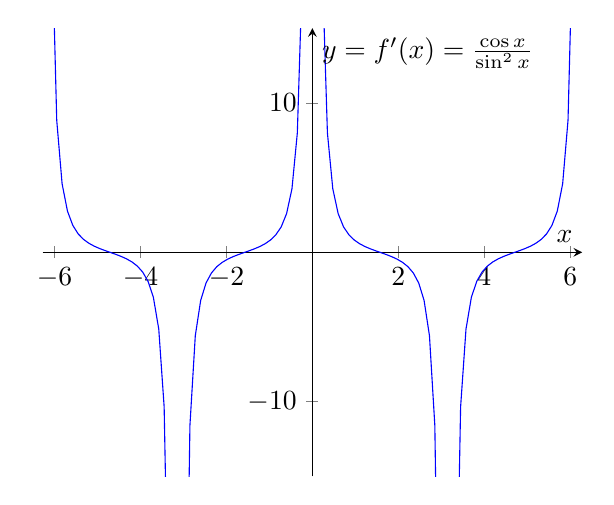
\begin{tikzpicture}
              \begin{axis}[
                axis lines = center,
                xlabel = $ x $,
                ylabel = {$ y = f'(x) = \frac{\cos x}{\sin^2 x} $},
                xmin = -6.28, xmax = 6.28,
                ymin = -15, ymax = 15
              ]
                \addplot[domain = -6.20:-3.20, color = blue] {cot(deg(x)) * 1/sin(deg(x))};
                \addplot[domain = -3.10:-0.1, color = blue] {cot(deg(x)) * 1/sin(deg(x))};
                \addplot[domain = 0.1:3.10, color = blue] {cot(deg(x)) * 1/sin(deg(x))};
                \addplot[domain = 3.20:6.20, color = blue] {cot(deg(x)) * 1/sin(deg(x))};
              \end{axis}
            \end{tikzpicture}}
  \question It is known that $ \Phi $ is a function such that:
            \begin{itemize}
              \item $ \Phi $ has a stationary point at $ x = 0 $.
              \item $ \od[2]{\Phi}{x} = 60x^4 - 180x^2 + 48 $.
              \item $ \Phi(2) = 0 $.
            \end{itemize}
    \begin{parts}
      \part Describe the nature of the stationary point at $ x = 0 $.
      \part Find the locations of the other stationary points.
      \part Find an exact expression for $ \Phi(x) $.
    \end{parts}
\end{questions}

\end{document}
